\chapter{Background}
% In this chapter, we review the concept of Turing Machines and constructing a parser for a programming language.

\section{Turing Machine}
% In this section, we review the definition of Turing Machines and executing a TM on a valid tape.

A \emph{Turing Machine} (TM) is a collection $(Q, \Sigma, \delta, q_0)$, where:
\begin{itemize}
    \item $Q$ is a set of states, including the accept state $A$ and reject state $R$;
    \item $\Sigma$ is the set of letters, which does not include the \texttt{blank} symbol;
    \item $\delta \colon Q \setminus \{A, R\} \times \Sigma^+ \to Q \times \Sigma^+ \times \{\texttt{left}, \texttt{right}\}$, where $\Sigma^+ = \Sigma \cup \{\texttt{blank}\}$, is the transition function; and
    \item $q_0 \in Q$ is the starting state.
\end{itemize}
Although based on Turing's work on \cite{turing1936computable}, this definition, along with others in this section, have been adapted from \cite{hopcroft2001automata}.

\begin{figure}[htb]
    \centering
    \begin{subfigure}{0.45\textwidth}
        \centering
        \begin{tikzpicture}
            \node[state, accepting] (q0) at (0, 0) {$q_0$};
            \node[state] (q1) at (2.5, 0) {$q_1$};
            \node[state, fill=green, opacity=0.6] (A) at (5, -1) {$A$};
            \node[state, fill=red, opacity=0.6] (R) at (5, 1) {$R$};
    
            \draw[->] (q0) edge[loop above] node[text width=1.5cm, align=center] {$0 \to 0, R$ $1 \to 1, R$} (q0);
            \draw[->] (q0) -- node[above] {$\# \to \#, L$} (q1);
            \draw[->] (q1) -- node[below, rotate=-20] {$0 \to \#, L$} (A);
            \draw[->] (q1) -- node[above, rotate=20, text width=1.5cm, align=center] {$1 \to 1, L$ $\# \to \#, L$} (R);
        \end{tikzpicture}
        \caption{Full notation}
    \end{subfigure}
    \hfill
    \begin{subfigure}{0.45\textwidth}
        \centering
        \begin{tikzpicture}
            \node[state, accepting] (q0) at (0, 0) {$q_0$};
            \node[state] (q1) at (2.5, 0) {$q_1$};
            \node[state, fill=green, opacity=0.6] (A) at (5, -1) {$A$};
            \node[state, fill=red, opacity=0.6] (R) at (5, 1) {$R$};
    
            \draw[->] (q0) edge[loop above] node {$0|1, R$} (q0);
            \draw[->] (q0) -- node[above] {$\#, L$} (q1);
            \draw[->] (q1) -- node[below, rotate=-20] {$0 \to \#, L$} (A);
            \draw[->] (q1) -- node[above, rotate=20] {$1|\#, L$} (R);
        \end{tikzpicture}
        \caption{Shorthand notation}
    \end{subfigure}
    \caption{A FSM representation of a TM that accepts binary numbers divisible by 2.}
    \label{fig:tm_isDiv2}
\end{figure}

We can represent a TM as a finite state machine (FSM). This is a directed graph, with vertices as states and edges as transitions. An example is given in Figure \ref{fig:tm_isDiv2}. In this case, the alphabet $\Sigma = \{0, 1\}$. The blank symbol is denoted by $\#$. The initial state is denoted by $q_0$; the accept state $A$ and the reject state $R$. Every edge corresponds to an evaluation of the transition function $\delta$, e.g. $\delta(q_1, 0) = (A, \texttt{blank}, \texttt{left})$. 

The figure presents two ways of representing FSM- subfigure (a) shows how all the transitions can be specified, while subfigure (b) only shows the transitions where the tapehead value is getting changed. We will make use of the shorthand FSM representation from now.

Let $\Sigma$ be an alphabet. A \emph{tape $T$ on $\Sigma$} is a function $T\colon \mathbb{Z} \to \Sigma^+$. In particular, the tape has infinite entries in both directions. Moreover, $T$ is a \emph{valid tape} if only finitely many symbols on $T$ are not \texttt{blank}, and all the values that can be non-\texttt{blank} are non-\texttt{blank}. That is, there exist integers $a, b$ such that for all $x \in \mathbb{Z}$, $T(x)$ is not \texttt{blank} if and only $x \geq a$ and $x \leq b$. 

We can represent a tape using a figure. For instance, let $\Sigma = \{0, 1\}$, and let $T$ be the tape on $\Sigma$ given below:
\[T(x) = \begin{cases}
    0 & x \in \{0, 2, 3\} \\
    1 & x \in \{1\} \\
    \texttt{blank} & \text{otherwise}.
\end{cases}\]
Then, the following figure represents the tape $T$:
\begin{figure}[H]
    \centering
    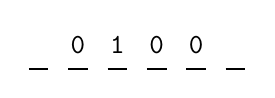
\begin{tikzpicture}
        \draw[thick] (-0.25, 0) -- (0, 0);
        \foreach \x[count=\i] in {0, 1, 0, 0} {
            \draw[thick] (\i*0.5-0.25, 0) -- (\i*0.5, 0);
            \node at (\i*0.5-0.125, 0.3) {\texttt{\x}};
        }
        \draw[thick] (2.25, 0) -- (2.5, 0);
    \end{tikzpicture}
\end{figure}
We will assume that the first non-blank value is at index 0.

A TM can be executed on a tape. Let $M$ be a TM with alphabet $\Sigma$, and let $T$ be a (valid) tape on $\Sigma$. We execute $M$ on $T$ inductively, as follows:
\begin{itemize}
    \item At any point during execution, we maintain 3 objects- a tape on $\Sigma$, a state in $M$ and an index in the tape (called the \emph{tapehead index}). 
    \item At the start, the tape is $T$; the tapehead index is $0$; and the state is the initial state $q_0$. 
    \item At some point during the execution, assume that we have the tape $S$, tapehead index $j$, with \emph{tapehead value} $T(j) = t$, and a non-terminating state $q$ (i.e. not $A$ or $R$). Denote $\delta(q, t) = (q', t', \texttt{dir})$. Then, the next state is $q'$, and the next tape $S'$ and the next tapehead index $j'$ are given by:
    \[S'(x) = \begin{cases}
        t' & x = i \\
        S(x) & \text{otherwise},
    \end{cases} \qquad j' = \begin{cases}
        j+1 & \texttt{dir} = \texttt{right} \\
        j-1 & \texttt{dir} = \texttt{left}.
    \end{cases}\]
    If the state $q'$ is not a terminating state, then the execution continues with these 3 objects. Otherwise, execution is terminated with terminating state $q'$.
\end{itemize}

\section{Parser}
TODO